%! Author = francis
%! Date = 30.10.20


\subsection{Simulated Method of Moments}
This method is suggested by Oh and Patton (2013).
In this setting, rank correlation e.g. Spearman's $\rho$ or Kendall's $\tau$,
and quantile dependence measures at different levels $\lambda_q$
are calibrated against their empirical counterparts.\medskip

Spearman's rho, Kendall's tau, and quantile dependence of a pair $(X,Y)$
with copula $C$ are defined as
\begin{align}
  \rho_S &= 12 \int\int_{I^2} C_{\bm{\theta}}(u,v)\, \dd u\, \dd v-3\label{eq:rho_S}\\
  \tau_K &= 4\mathbb{E}[C_{\bm{\theta}}\{F_X(x), F_Y(y)\}]-1,\\
  \lambda_q &=
  \begin{cases}
    \p(F_X(X)\leq q| F_Y(Y)\leq q) = \displaystyle \frac{C_{\bm{\theta}}(q,q)}{q},
    &\text{ if } q\in (0,0.5],\\
    \p(F_X(X)>q|F_Y(Y)>q) =\displaystyle \frac{1-2q+C_{\bm{\theta}}(q,q)} {1-q},
    &\text{ if } q\in (0.5,1).
  \end{cases}
\end{align}\medskip
The empirical counterparts are
\begin{align*}
  \hat\rho_S &= \frac{12}{n} \sum_{k=1}^n \hat F_X(x_k) \hat F_Y(y_k)
               -3,\\
  \hat\tau_K &= \frac{4}{n}\sum_{k=1}^n \hat{C}\{\hat{F}_X(x_i),\hat{F}_X(y_i)\} -1 ,\\
  \hat\lambda_q &=
                  \begin{cases}
                    \displaystyle\frac{1}{n} \sum_{k=1}^n \frac{\1_{\{\hat
                        F_X(x_k)\leq q, \hat F_Y(y_k)\leq q\}}} {q},
                    &\text { if } q\in (0, 0.5],\\
                    \displaystyle \frac{1}{n} \sum_{k=1}^n
                    \frac{\1_{\{\hat F_X(x_k)>q, \hat F_Y(y_k)>q\}}}
                    {1-q}, &\text { if } q\in (0.5,1).
                  \end{cases},
\end{align*}
where $\hat{F}(x) := \frac{1}{n}\sum_{k=1}^n 1_{\{x_i\leq x\}}$ and
$\hat{C}(u,v) := \frac{1}{n}\sum_{k=1}^n 1_{\{u_i\leq u, v_i\leq v\}}$.\medskip

We denote $\tilde{\bm{m}}(\bm{\theta})$ be a $m$-dimensional vector of dependence measures according the the
dependence parameters $\bm{\theta}$,and  $\hat{\bm{m}}$ be the corresponding empirical counterpart.
The difference between dependence measures and their counterpart is denoted by
\begin{align*}
    \bm{g}(\bm{\theta}) = \hat{\bm{m}} - \tilde{\bm{m}}(\bm{\theta}).
\end{align*}\medskip

The SMM estimator is
\begin{align*}
    \hat{\bm{\theta}} = \argmin_{\bm{\theta}\in \bm{\Theta}} \bm{g}(\bm{\theta})^\intercal
    \hat{\bm{W}}
     \bm{g}(\bm{\theta}),
\end{align*}
where $\hat{W}$ is some positive definite weigh matrix.\medskip

In this work, we use $\tilde{\bm{m}}(\bm{\theta}) = (\rho_S, \lambda_{0.05}, \lambda_{0.1},
\lambda_{0.9}, \lambda_{0.95})^\intercal$
for calibration of Bitcoin price and CME Bitcoin future.

\subsection{Maximum Likelihood Estimation}
The MLE estimator for a bivariate parametric copula is
\begin{align}
    \hat{\bm{\theta}} = \argmax_{\bm{\theta} \in \bm{\Theta}} l(X,Y; \bm{\theta}), \label{eq:EMLE}
    \end{align}
where
\begin{align}
    l(X,Y; \bm{\theta}) = \sum_{k=1}^n \log c(x_i, y_i;\bm{\theta}). \label{eq:Likelihood}
    \end{align}\medskip

Procedure of maximising equation~\ref{eq:EMLE} as a whole is called exact maximum likelihood method.
Leveraging the attractive feature of copula that one can model the dependence structure and marginals separately,
we rewrite~\ref{eq:Likelihood} into canonical expression
\begin{align}
    l(X,Y; \bm{\theta}) = \sum_{k=1}^n \log c\{F_X(x_i; \delta_X), F_Y(y_i; \delta_Y); \bm{\gamma}\}
    + \sum_{k=1}^n \log f_X(x_i; \bm{\delta}_X) + \sum_{k=1}^n \log f_X(y_i; \bm{\delta}_Y),
    \end{align}
where the $\bm{\gamma}$ is the dependence parameter in the copula and $\bm{\delta}$ is the parameters in the margins.\medskip

The inference-functions for margins (IFM) approach by Joe is a two step procedure of maximising~\ref{eq:EMLE}.
The approach calibrate first the $\bm{\delta}$s and then the  $\bm{\gamma}$.\medskip

Similar to the IFM approach, pseudo-maximum likelihood approach by Genest and Rivest (1993) replace the parametric margins by
empirical estimates, we rewrite \ref{eq:Likelihood} again with
\begin{align}
    l(X,Y; \bm{\theta}) = \sum_{k=1}^n \log c(u_i, v_i;\bm{\gamma}),
    \end{align}
where $u_i = \hat{F}_X(x_i)$ and $v_i = \hat{F}_Y(y_i)$.

\subsection{Comparison}
Both the simulated method of moments and the maximum likelihood estimation are unbiased and
proven to give good fits (ref ...).
The problem remain is which procedure is more suitable for hedging.
%Cryptocurrencies are known to be very volatile.
Sample and fitted quantile dependence for Bitcoin and CME future.

\begin{figure}[h]
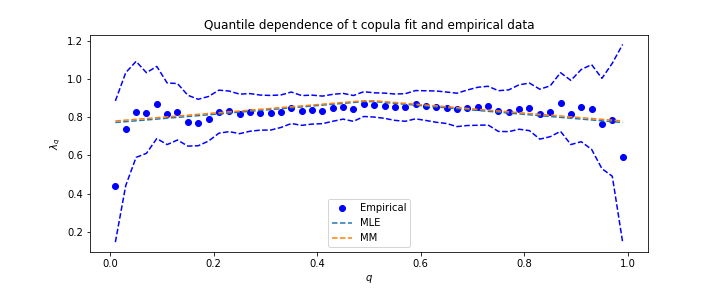
\includegraphics[width=\textwidth]{_pics/t Copula quantile dependence.png}
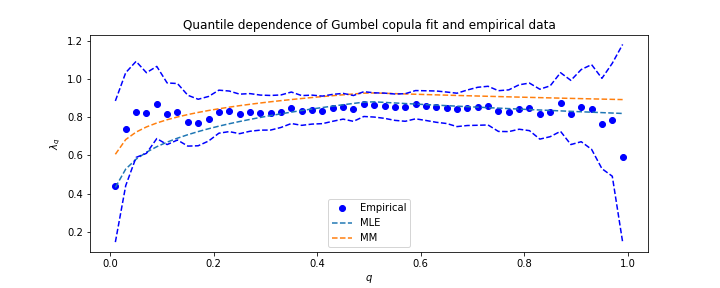
\includegraphics[width=\textwidth]{_pics/Gumbel Copula quantile dependence.png}
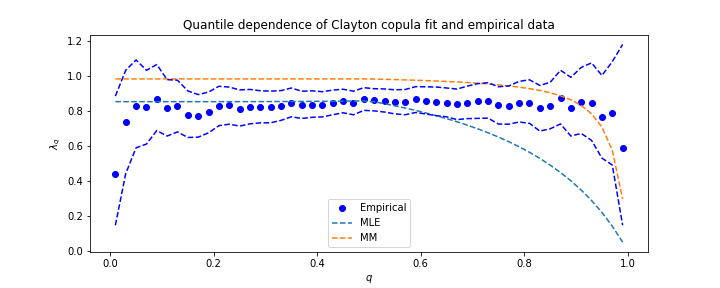
\includegraphics[width=\textwidth]{_pics/Clayton Copula quantile dependence.png}
  \caption{}
\label{fig:quantile dependence1}
\end{figure}


The MM estimation perform just as we decided: match the upper and quantile dependence.




%
%
%\subsection{Two-Stage Estimation}\label{subsec:two-stage-estimation}
%~\cite{joe2005asymptotic} study the efficiency of a two-stage estimation procedure of copula estimation.
%The authors also call this method inference function for margins IFM.
%
%\textbf{Pros}
%\begin{enumerate}
%    \item Almost as efficient as MLE methods but easier to be implemented
%    \item Yields an asymptotically Gaussian, unbiased estimate
%\end{enumerate}
%
%\textbf{Cons}
%\begin{enumerate}
%    \item Subject to specification of marginals \cite{kim2007comparison}
%\end{enumerate}
%
%Our data
%\begin{align}
%    \pmb{y} = \begin{bmatrix}
%                  y_{11} & \cdots & y_{1i}\\
%                  \vdots & \ddots & \vdots \\
%                  y_{n1} & \cdots & y_{ni}
%                  \end{bmatrix}
%    \end{align}
%Let $F$ and $f$ be the joint cdf and joint density of $\pmb{y}$ with parameters $\pmb{\delta}$,
%and let $F_i$ and $f_i$ be the marginal cdf and marginal density for the $i^\text{th}$ random variable with parameters $\pmb{\theta}_i$, we have
%\begin{align}
%    f(\pmb{y}; \pmb{\theta}_1, \pmb{\theta}_2,\dots \pmb{\theta}_i, \pmb{\delta}) =
%    c\{F_1(\pmb{y}_1;\pmb{\theta}_1), F_2(\pmb{y}_2; \pmb{\theta}_2), \dots, F_i(\pmb{y}_1;\pmb{\theta}_i); \pmb{\delta}\}
%    \prod^i_{j=1}f_i(\pmb{y}_j;\pmb{\theta}_j)
%    \end{align}
%
%For a sample of size $n$, the log-likelihood of functions of the $i^\text{th}$ univariate margin is
%\begin{align}
%    L_i(\theta_i) = \sum^n_{m=1} \log f_i(y_{mi}; \theta_i),
%    \end{align}
%
%and the log-likelihood function for the joint distribution is
%\begin{align}
%    L(\delta, \theta_1, \theta_2, \dots, \theta_i) = \sum^n_{m=1}\sum^i_{j=1} \log f(y_{mj}; \delta, \theta_1, \theta_2, ..., \theta_i)
%    \end{align}
%
%In most cases, one does not have closed form estimators and numerical techniques are needed.
%Numerical ML estimation difficulty increase when the total number of parameters increases.
%The two-stage estimation is designed to overcome this problem.
%
%The two-stage procedure is
%\begin{enumerate}
%    \item estimate the univariate parameters from separate univariate likelihoods to get $\tilde{\pmb{\theta}_1}, ..., \tilde{\pmb{\theta}_i}$
%    \item maximize $L(\pmb{\delta}, \tilde{\pmb{\theta}_1}, \dots, \tilde{\pmb{\theta}_i})$ over $\pmb{\delta}$ to get $\tilde{\pmb{\delta}}$
%    \end{enumerate}
%
%Under regularity conditions
%\footnote{Regularity conditions include
%1. $\exists \frac{\partial \log f(x;\theta)}{\partial \theta}, \frac{\partial^2 \log f(x;\theta)}{\partial \theta^2}, \frac{\partial^3 \log f(x;\theta)}{\partial \theta^3}$ for all $x$;
%2. $\exists g(x), h(x) and H(x)$ such that for $\theta$ in a neighborhood $N(\theta_0)$ the relations
%$\left|\frac{\partial f(x;\theta)}{\partial theta}\right| \leq g(x)$,
%$\left|\frac{\partial^2 f(x;\theta)}{\partial \theta^2}\right| \leq h(x)$,
%$\left|\frac{\partial^3 f(x;\theta)}{\partial \theta^3}\right| \leq H(x)$ hold for all $x$, and
%$\int g(x) dx < \infty$, $\int h(x) dx < \infty$, $\mathbb{E}_\theta \{H(X)\} < \infty$ for $\theta \in N(\theta_0)$;
%3. For each $\theta \in \Theta$, $0< \mathbb{E}_\theta \left\{
%\left(
%\frac{\partial \log f(X;\theta)}{\partial \theta}
%\right)^2
%\right\}$. For detail see section 4.2.2 of~\cite{serfling2009approximation}}
%, $(\pmb{\tilde{\theta}}_1,\dots \pmb{\tilde{\theta}}_i, \pmb{\tilde{\delta}})$ is the solution of
%\begin{align}
%    (\partial L_1 / \partial \pmb{\theta}^\intercal_1,
%    \dots, \partial L_i / \partial \pmb{\theta}^\intercal_i, \partial L / \partial \pmb{\pmb{\delta}}^\intercal_1) = \pmb{0}
%    \end{align}
%
%For comparison, if we optimize $L$ directly without the two-stage procedure (i.e.~MLE), we solve for
%\begin{align}
%    (\partial L / \partial \pmb{\theta}^\intercal_1,
%    \dots, \partial L / \partial \pmb{\theta}^\intercal_i, \partial L / \partial \pmb{\pmb{\delta}}^\intercal_1) = \pmb{0}
%    \end{align}
%
%We denote the two solutions as
%$\tilde{\pmb{\eta}} = (\pmb{\tilde{\theta}}_1,\dots \pmb{\tilde{\theta}}_i, \pmb{\tilde{\delta}})$ for two-stage procedure;
%$\hat{\pmb{\eta}} =(\pmb{\hat{\theta}}_1,\dots \pmb{\hat{\theta}}_i, \pmb{\hat{\delta}})$ for MLE procedure.
%and compare the asymptotic relative efficiency of $\tilde{\pmb{\eta}}$ and $\hat{\pmb{\eta}}$.
%
%Asymptotics: yet to be done.\\
%~\cite{kim2007comparison} show the estimation of $\pmb{\theta}$ may be seriously affected.
%They compare the two-stage approach and Canonical Maximum Likelihood Method by simulation and
%conclude that Canonical Maximum Likelihood is prefered from a computational statistics and data analysis point of view.
%
%\subsection{Canonical Maximum Likelihood Method}\label{subsec:canonical-maximum-likelihood-method}
%This approach was studied by~\cite{genest1995semiparametric} and~\cite{shih1995inferences}.
%One estimates the margins using empirical CDF
%\begin{align}F_X(x)=\frac{1}{n+1}\sum_{i=1}^n 1(X_i \leq x)\end{align},
%
%we maximize the log-likelihood
%\begin{align}
%    L(\delta) = \sum_{i=1}^n \log [c_\delta \{F_X(X_i), F_Y(Y_i)\}]
%    \end{align}
%
%This procedure does not require specification of marginals.
%
%
%
%
%
%%also by Wang and Ding, 2000; Tsukahara, 2005
%%This is also known as pseudo maximum likelihood (PML) and as canonical maximum likelihood (see Cherubini et al., 2004)
%%
%%Genest and Werker (2002) obtained conditions under which the PMLE is asymptotically efficient.
%%
%%
